\documentclass[class=article, crop=false]{standalone}
\usepackage[subpreambles=true]{standalone}
\usepackage{import}
\usepackage{preamble}
\usepackage{pdfpages}
\begin{document}
\section{Endogeneity}
\label{sec:endogeneity}
The above decompositions focus primarily on outright pay discrimination. However, we have seen that occupational clustering occurs in almost all ethnic groupings, putting downwards pressure on the pay of males (but not females). One reason this may exist is due to differences in preferences; if minorities prefer not to work in particular industries, then we would expect to see a relatively higher wage premium for minorities working in such industries. However, observing Figures \ref{fig:m_wpremium-percnonwhite} and \ref{fig:f_wpremium-percnonwhite} for males and females respectively, there is very little correlation (if any) between the percentage of non-White workers in an industry and the wage premium. This implies that there is little evidence of preferences causing the occupational clustering - or, if there it is due to preferences, then workers are not being compensated accordingly.

Therefore, it would be useful to explore whether the clustering is indicative of other discriminatory effects, namely institutional and statistical discrimination, as discussed in Section \ref{sec:Stat_discrim and signalling}. If workers perceive that an industry is particularly \enquote{racist} then they may avoid it - the clustering for males is particularly of interest as it occurs at a cost of lower remuneration. Even if employers themselves are not racist, minorities may choose to avoid such industries which have historically undervalued (or currently undervalue) the productivity of minorities; perceptions regarding the quality of workers could act as a barrier to entry, discouraging minorities. This is not seen in Figure \ref{fig:cross_correls}, with no correlation between racist attitudes and the wage premium and proportion of non-White workers of either sex. 

There are two reasons explaining this. Firstly, the survey of \enquote{British-ness} attitudes from the \acrlong{us} dataset could be a poor indicator of racist attitudes. Levels of reported racist incidents are available but suffer from a poor sample size. Thus, analysis using a more accurate proxy may yield alternative results. Secondly, the data uses industry rather than occupation data due to the incompatibility of 1992 and 2007 occupational codes. Finally, since Figures \ref{fig:explained_male_stacked} and \ref{fig:explained_female_stacked} outlined that education was a positive factor influencing the wages of all minorities, both male and female, it could be that male minorities have high levels of education yet employers undervalue their quality/productivity.

Therefore, the dataset provides no clear indication of why occupational clustering occurs. Given the importance of occupational clustering in determining wages, as discussed in Section \ref{sec:explained_diff}, future research into this will provide valuable insights into how policy can address the pay gap.

%"Could be that the proxy is bad. Or that the barrier is not racism, something else. Could be perceptions of their quality."
%\import{graphs/}{wpremium-percracist}
%\begin{comment}
\begin{figure}
    \caption{Cross-correlations of indicators, coloured by industry group}
    \begin{subfigure}[t]{\textwidth}
        \centering
        \vspace{-100pt}
        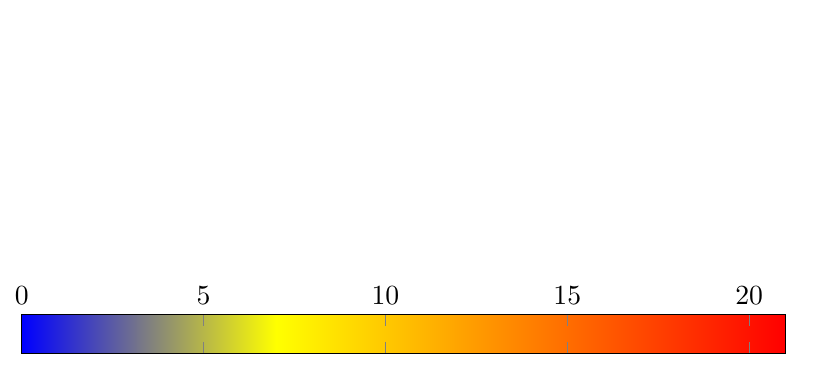
\begin{tikzpicture}
        \hspace{-8pt}
        \begin{axis}[
        hide axis,
        scale only axis,
        colorbar horizontal,
        point meta min=0,
        point meta max=21,
        colorbar style={
            width=0.8\textwidth,
            xtick={0,5,...,21},
            ylabel style={},
            xticklabel pos=upper,
            at={(0.0,0.0)},anchor=north west
            }
         ]
        \addplot[draw=none] coordinates {(0,0)};
        \end{axis}
        \end{tikzpicture}
    \end{subfigure}
    %Male ----------------------------------
    \begin{subfigure}{0.3\textwidth}
        \import{graphs/}{m_wpremium-percnonwhite}
        \caption{Male}
        \label{fig:m_wpremium-percnonwhite}
    \end{subfigure}
    \begin{subfigure}{0.3\textwidth}
        \import{graphs/}{m_wpremium-percracist}
        \caption{Male}
        \label{fig:m_wpremium-percracist}
    \end{subfigure}
    \begin{subfigure}{0.3\textwidth}
    \centering
        \import{graphs/}{m_percnonwhite-percracist}
        \caption{Male}
        \label{fig:m_percnonwhite-percracist}
    \end{subfigure}
    %\begin{subfigure}{0.1\textwidth}
     %   \hfill
    %\end{subfigure} 
    %Female ----------------------------------
    \begin{subfigure}{0.3\textwidth}
        \import{graphs/}{f_wpremium-percnonwhite}
        \caption{Female}
        \label{fig:f_wpremium-percnonwhite}
    \end{subfigure}
    \begin{subfigure}{0.3\textwidth}
        \import{graphs/}{f_wpremium-percracist}
        \caption{Female}
        \label{fig:f_wpremium-percracist}
    \end{subfigure}
    \begin{subfigure}{0.3\textwidth}
    \centering
        \import{graphs/}{f_percnonwhite-percracist}
        \caption{Female}
        \label{fig:racist_nonwhite}
    \end{subfigure}
    %\begin{subfigure}{0.1\textwidth}
     %   \hfill
    %\end{subfigure} 
    \label{fig:cross_correls}
\end{figure}
%\end{comment}

\end{document}